\documentclass[utf8,oneside]{ctexbook} % 中文支持,oneside代表书籍不按奇偶页数分别处理
\usepackage{amsmath} % 数学公式支持
\usepackage{fancyhdr} % 页眉页脚支持
\usepackage{graphicx} % 图片支持
\usepackage{geometry} % 版面(页边距、纸张大小)设置支持
\usepackage{hyperref} % 超链接支持
\usepackage{titling} % maketitle 格式设置支持

% CTeX 宏包设置
\ctexset {
    chapter = {
        % 设置 chapter 的标题格式
        format = \huge\bfseries\centering,
        % 设置 chapter 编号的前缀和后缀
        name = {,.},
        % 设置 chapter 编号的样式
        number = \Roman{chapter},
        % 取消目录分页
        break = {},
    },
    % 设置目录标题
    contentsname = {},
}

% maketitle 格式设置
\pretitle{\centering \Huge \textbf}
\posttitle{\par \vspace{0.5cm}}
\preauthor{\centering \Large \textit}
\postauthor{\par \vspace{0.5cm}}
\predate{\centering}
\date{}
\postdate{
    % 校名校徽
    \begin{center}
        \vspace{6cm}
        % 校名
        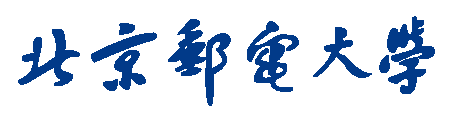
\includegraphics[width = .43\textwidth]{pic/BUPT/BUPT_name.eps}\\
        \vspace{1cm}
        % 校徽
        
\includegraphics[width = .23\textwidth]{pic/BUPT/BUPT_Logo.eps}\\
    \end{center}
}

% 基本信息
\title{概率论与随机过程习题解答}
\author{计算机学院(国家示范性软件学院)\\吴政隆}
\date{\today}

% 设置页眉页脚内容
\pagestyle{fancy}
\lhead{} \chead{\textit{\thetitle}} \rhead{}
\lfoot{} \cfoot{\thepage} \rfoot{}

% 设置纸张大小
\geometry{a4paper}

% 设置页边距
% \geometry{left=1cm,right=1cm,top=1cm,bottom=1cm}

% 文档内容
\begin{document}

% 标题
\maketitle

% Chapter_0 版权声明、前言和目录
% Chapter_0

% 版权信息

\section*{版权声明}

本文档“概率论与随机过程习题解答”(以下简称“本文档”)的作者为吴政隆(WU Zhenglong,常用网络用户名为 itdevwu)。本文档的著作权归属于作者所有。

在未经特别说明的情况下,本文档的内容(包括但不限于文字、图片等)采用“\href{https://creativecommons.org/licenses/by-sa/4.0/deed.zh}{知识共享署名-相同方式共享 4.0 国际许可协议} ”(简称为“CC-BY-SA 4.0 协议”)进行许可。该协议由\href{https://creativecommons.org/}{知识共享组织(Creative Commons)}撰写。请注意,本作品中注明以其他方式进行许可或著作权人非本文档作者的内容,需按照特殊说明进行处理。在大多数情况下,这意味着您在遵循以下义务:

\begin{itemize}
    \item \textbf{署名}——您必须给出适当的署名,提供指向本许可协议的链接,同时标明是否(对原始作品)作了修改。您可以用任何合理的方式来署名,但是不得以任何方式暗示许可人为您或您的使用背书;
    
    \item \textbf{相同方式共享}——如果您再混合、转换或者基于本作品进行创作,您必须基于与原先许可协议相同的许可协议分发您贡献的作品;
    
    \item \textbf{没有附加限制}——您不得用法律术语或者技术措施限制他人做许可协议允许的事,
    
\end{itemize}

\noindent 的同时,拥有了以下权利:

\begin{itemize}
    \item \textbf{共享}——在任何媒介以任何形式复制、发行本作品;
    
    \item \textbf{演绎}——以任何(包括商业)用途为目的,修改、转换或以本作品为基础进行创作。
    
\end{itemize} 

只要您遵守许可协议条款,许可人就无法收回您的上述权利。

“CC-BY-SA 4.0 协议”所授予的权利不一定包括您所想获得的全部权利。比如,法律赋予作者的其他权利,如肖像权、隐私权或姓名权等,可能会限制您使用作品的方式。

需要注意的是,上述内容是对“CC-BY-SA 4.0 协议”的易读概括,不能替代该协议的法律文本。您可以在知识共享(Creative Commons)组织的官方网站获取上述协议的法律文本。例如,“CC-BY-SA 4.0 协议”的官方中文法律文本位于:\href{https://creativecommons.org/licenses/by-sa/4.0/legalcode.zh-Hans}{creativecommons.org/licenses/by-sa/4.0/legalcode.zh-Hans} 。当上述概括的内容与法律文本发生冲突时,以法律文本为准。

有时,作者也会用下列图标表示对内容以“CC-BY-SA 4.0 协议”进行许可:

\begin{center}
    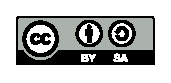
\includegraphics[width = 0.3\textwidth]{pic/CC-BY-SA/BY-SA.eps}
\end{center}

本文档采用 \LaTeX 撰写。这意味着作者在撰写本文档内容的同时还撰写了一份软件源代码,以处理本文档内容的排版、渲染等问题。

“CC-BY-SA 4.0 协议”具有对由\href{https://www.fsf.org/}{自由软件基金会(Free Software Foundation, Inc)}提供的“\href{https://www.gnu.org/licenses/gpl-3.0.html}{GNU GENERAL PUBLIC LICENSE Version 3}”(以下简称“GPLv3协议”)的单向兼容性。这意味着如果您希望在本书的 \TeX 代码的基础上进行再创作和分发,您亦可遵循“GPLv3协议”。在中国大陆,由工业和信息化部信息化和软件服务业司指导,挂靠在中国电子技术标准化研究院的\href{https://www.coscl.org.cn/}{中国开源云联盟(COSCL)},撰写了“\href{https://license.coscl.org.cn/MulanPubL-2.0/index.html}{木兰公共许可证,第2版}”(以下简称“MulanPubL-2.0协议”)。其具有与“GPLv3协议”相似的特性,并对中华人民共和国的法律术语进行了针对性说明。您亦可以根据自己的需要,在本书的 \TeX 代码的基础上进行再创作和分发时,选择使用“MulanPubL-2.0协议”进行分发。

请注意,上述说明基于“CC-BY-SA 4.0 协议”本身的兼容性,不代表本文档的代码采用“GPLv3协议”或“MulanPubL-2.0协议”进行授权或分发。

对于不同协议,作者的建议大致如下:

\begin{itemize}
    \item 如果您希望使用本文档的内容或者文件本身(即代码编译后的二进制文件,包括但不限于.pdf,.ps,.div等格式),遵循“CC-BY-SA 4.0 协议”是更好的选择;
    
    \item 如果您希望在 \TeX 代码(包括但不限于.tex,.sty等格式)的基础上进行再创作和分发,遵循“GPLv3协议”或“MulanPubL-2.0协议”是更好的选择。
\end{itemize}

本声明的最终解释权属于作者。

% 前言

\newpage
\section*{前言}

“概率论与随机过程”是北京邮电大学计算机类学生在大二秋季学期的“二选一”课程之一。这门课程对于数据科学、深度学习等方向的后续学习都十分重要。

在北京邮电大学,该课程的教材是由理学院数学系张丽华副教授和周清教授编纂的《\textit{Probability and Stochastic Processes}》。由于在大部分学校,随机过程都是单独开课,且北邮所使用的教材是本校自编的英文教材,导致课程学习资料匮乏。考虑到本课程的重要意义,作者希望将学习过程的习题解法加以整理,以期惠及后人。

为了方便读者反馈,改进本文档内容,用于生成本文档的 \TeX 代码会被托管在 GitHub 网站上的 \href{https://github.com/itdevwu/BUPT-Probability-and-Stochastic-Processes}{itdevwu/BUPT-Probability-and-Stochastic-Processes} 这一 repo 中。读者可以通过提 issue 和 pull request 等方式来参与到本文档的编修工作中。

受限于作者的知识水平和细致程度,本文档无法做到尽善尽美。恳请各位斧正。

% 水平方向靠右侧对齐
\begin{flushright}
    % 竖直方向靠下对齐
    \vfill \textit{
        北京邮电大学\\
        \theauthor
    }
\end{flushright}


% 目录

\newpage
\section*{目录}
\vspace{-3cm}
\tableofcontents


% Chapter_1 Events and Their Probabilities
% BUPT-Probability-and-Stochastic-Processes (c) by Zhenglong WU(itdevwu)

% BUPT-Probability-and-Stochastic-Processes has a Chinese name "概率论与随机过程习题解答".

% BUPT-Probability-and-Stochastic-Processes is licensed under a
% Creative Commons Attribution-ShareAlike 4.0 International License.

% You should have received a copy of the license along with this
% work. If not, see <http://creativecommons.org/licenses/by-sa/4.0/>.

\chapter{Events and Their Probabilities}
\newpage % 由于此前设置 chapter 标题后不换页,此处换页

\section{Exercises Solution}

\subsection{Experiment, Sample Space and Random Event}

% 1.1
\paragraph{1.1}
We consider the following random experiment: a fair die is rolled; if (and only if) a 6 is obtained, the die is rolled a second time. How many elementary outcomes are there in the sample space $\Omega$?
 
\solution
If the first roll obtained $k\in \{1,2,3,4,5\}$, \par
than the result set would be $\mathbf{A} = \{1,2,3,4,5\}$,\par
else, there would be a second roll that obviously have 6 results.\par
Thus, $card(\Omega) = card(\mathbf{A}) + 6 = 11$.

% 1.2
\paragraph{1.2}
An academic department has just completed voting by secret ballot for a department head. The ballot box contains four slips with votes for candidate A and three slips with votes for candidate B. Suppose that these slips are removed from the box one by one.
\begin{itemize}
    \item[(a)] List all possible outcomes.
    \item[(b)] Suppose that a running tally is kept as slips are removed. For what outcomes does A remain ahead of B throughout the tally?
\end{itemize}

\solution
(a) Consider combinations and permutations:

When slips for B are continuous: $C_{5}^{1}$.

When 2 of slips for B are continuous and the other is not: $A_{5}^{2}$.

When none of slips for B are not continuous: $C_{5}^{3}$.

Thus there should be $C_{5}^{1}+A_{5}^{2}+C_{5}^{3} = 5+20+10 = 35$ outcomes:
\begin{equation*}
    \begin{split}
      \{& AAAABBB, AAABABB, AAABBAB, AAABBBA, AABAABB,\\
        & AABABAB, AABABBA, AABBAAB, AABBABA, AABBBAA,\\
        & ABAAABB, ABAABAB, ABAABBA, ABABAAB, ABABABA,\\
        & ABABBAA, ABBAAAB, ABBAABA, ABBABAA, ABBBAAA,\\
        & BAAAABB, BAAABAB, BAAABBA, BAABAAB, BAABABA,\\
        & BAABBAA, BABAAAB, BABAABA, BABABAA, BABBAAA,\\
        & BBAAAAB, BBAAABA, BBAABAA, BBABAAA, BBBAAAA\}
    \end{split}
\end{equation*}

(b)
$\{AAAABBB, AAABBAB, AABAABB, AABABAB, AABABBA\}$

% 1.3
\paragraph{1.3}
From 10 married couples, we want to select a group of people that is not allowed to contain a married couple.
\begin{itemize}
    \item[(a)] How many choices are there?
    \item[(b)] How many choices are there if the group must also consist of 3 men and 3 women?
\end{itemize}

\solution
(a)

Select 6 couples out of 10, then select 1 person from each couple.

Thus we have $C_{10}^6 {(C_{2}^1)}^6 = 210 \times 64 = 13440$.

(b)

Firstly we select 6 couples out of 10.

For "lady first", we select 3 couples out of previous 6, then select 1 female from each.

Other couples will be selected to choose male.

Therefore there will be nothing to choose from them.

Thus the answer is $C_{10}^6 C_{6}^3 = 210 \times 20 = 4200$.

% 1.4
\paragraph{1.4}
Consider n-digit numbers where each digit is one of the 10 integers $0, 1, \cdots ,9$. How many such numbers are there for which
\begin{itemize}
    \item[(a)] no two consecutive digits are equal?
    \item[(b)] 0 appears as a digit a total of $i$ times $i = 0,\cdots ,n?$
\end{itemize}

\solution
(a)

First digit must not be 0 and any digit cannot be the same as the previous one.

Thus the answer is ${(C_9^1)}^{10} = 9^{10} = 3486784401$.

(b)

Consider 0 appears $i$ times:

We select $i$ positions out of 9 for 0, the rest positions can be any digit except 0.

Thus we get $C_9^1 C_9^i (C_{9}^{1})^{9-i} = 9 C_9^i \cdot 9^{9-i} = C_9^i \cdot 9^{10-i}$ as answer.

(Calculation)

We can use Python or other numeric computing methods to calculate such formula.

\textit{\textbf{Note}: There is a possibility that the answer exceeds INT\_MAX during calculation.}

% 1.4的答案,允许在此处或底部浮动
\begin{table}[hb]
    \centering
    \resizebox{.95\textwidth}{!}{
        \begin{tabular}{|c|c|c|c|c|c|c|c|c|c|c|}
            \hline
            \textit{\textbf{i}}     & 0          & 1          & 2          & 3         & 4        & 5       & 6      & 7     & 8   & 9 \\ \hline
            \textit{\textbf{count}} & 3486784401 & 3486784401 & 1549681956 & 401769396 & 66961566 & 7440174 & 551124 & 26244 & 729 & 9 \\ \hline
        \end{tabular}
    }
\end{table}

\paragraph{1.5}
Let E,F,G be three events. Find expressions for the events that of E, G, F
\begin{itemize}
    \item[(a)] only F occurs,
    \item[(b)] both E and F but not G occur,
    \item[(c)] at least one event occurs,
    \item[(d)] at least two events occur,
    \item[(e)] all three events occur,
    \item[(f)] none occurs,
    \item[(g)] at most one occurs,
    \item[(h)] at most two occur.
\end{itemize}

\noindent \textit{\textbf{Notation}: Given a set $U$, $B$ is complement of $A$ in U, written $B = A \setminus U = A^C = U - A$.}

\solution

For two events $A, B$, there are:

\begin{center}
    $A\cup B$ is an event in which A OR B (or both) occur,\\
    $A\cap B = AB$ is an event in which A AND B occur,\\
    $A^C$ is an event in which A does not occur.
\end{center}

\begin{itemize}
    \item[(a)] $F[(E\cup G)^C]$
    \item[(b)] $(E\cup F)(G^C)$
    \item[(c)] $E\cup F\cup G$
    \item[(d)] $(EF)\cup (EG)\cup (FG)$
    \item[(e)] $EFG$
    \item[(f)] $(E\cup F\cup G)^C$
    \item[(g)] $[(EF)\cup (EG)\cup (FG)]^C$
    \item[(h)] $(EFG)^C$
\end{itemize}

\textit{\textbf{Note}: There are relationships between problem (c, d, e) \& problem (f, g, h).}


% Chapter_2 Random Variable
\chapter{Random Variable}
\newpage % 由于此前设置 chapter 标题后不换页,此处换页


% Chapter_3 Random Vectors
\include{chapters/Chapter_3/Chapter_3.tex}

% Chapter_4 Sequences of Random Variables
\include{chapters/Chapter_4/Chapter_4.tex}

% Chapter_5 Introduction to Stochastic Processes
\include{chapters/Chapter_5/Chapter_5.tex}

% Chapter_6 Stationary Processes
\include{chapters/Chapter_6/Chapter_6.tex}

% Chapter_7 Finite Markov Chains
% BUPT-Probability-and-Stochastic-Processes (c) by Zhenglong WU(itdevwu)

% BUPT-Probability-and-Stochastic-Processes has a Chinese name "概率论与随机过程习题解答".

% BUPT-Probability-and-Stochastic-Processes is licensed under a
% Creative Commons Attribution-ShareAlike 4.0 International License.

% You should have received a copy of the license along with this
% work. If not, see <http://creativecommons.org/licenses/by-sa/4.0/>.

\chapter{Finite Markov Chains}
\newpage % 由于此前设置 chapter 标题后不换页,此处换页


% Chapter_8 Independent-Increment Processes
\chapter{Independent-Increment Processes}
\newpage % 由于此前设置 chapter 标题后不换页,此处换页


\end{document}
